\documentclass[letterpaper,12pt]{report}

% == Packages ==========================================================

% Unused packages from Mackenzie's thesis
% \usepackage{amsmath}
% \usepackage{amssymb}
% \usepackage{amsfonts}
% \usepackage{lipsum}
% \usepackage{multicol}
% \usepackage{accents}
% \usepackage{wrapfig}
% \usepackage{euscript}
% \usepackage[linesnumbered,lined,boxruled,commentsnumbered]{algorithm2e}

% All inherited from Mackenzie
\usepackage{float}
\usepackage{tabularx}
\usepackage{latexsym}
\usepackage{color}
\usepackage{xcolor}
\usepackage{graphicx}
\usepackage{float}
\usepackage{subcaption}
\usepackage{epsfig}
\usepackage{hyperref}
\usepackage{setspace}
\usepackage{fancyhdr}
\usepackage{hyperref}
\usepackage[left = 1.5in, right = 1in, top = 1in, bottom = 1.25in, head = 0.5in]{geometry}
\usepackage{textcomp}
\usepackage{pdfpages}
\usepackage[acronym]{glossaries}
\usepackage{attachfile}

\graphicspath{{assets/}}

% https://tex.stackexchange.com/questions/55096/anti-aliasing-from-latex-to-pd
% Fixes some weird anti-aliasing issues when compiling locally with pdflatex
% that doesn't occur on Overleaf
\usepackage[utf8]{inputenc}
\usepackage[english]{babel}
\usepackage{lmodern}
\usepackage[T1]{fontenc}
\usepackage[babel=true]{microtype}

% Table support (using what Pandoc spits out).
\usepackage{booktabs}

% Pandoc uses tightlist for bullet lists, you can just do nothing
\def\tightlist{}

% Pandoc generates `passthrough' commands for inline code as described in 
% https://github.com/jgm/pandoc/issues/5696, we can just effectively ignore it
\newcommand{\passthrough}[1]{#1}

% Code listings. We use inconsolata for the font.
\usepackage{listings}
\usepackage{inconsolata}
\definecolor{codegreen}{rgb}{0,0.6,0}
\definecolor{codegray}{rgb}{0.5,0.5,0.5}
\definecolor{codepurple}{rgb}{0.58,0,0.82}
\definecolor{backcolour}{rgb}{0.95,0.95,0.92}

\lstset{
    backgroundcolor=\color{backcolour},   
    commentstyle=\color{codegreen},
    keywordstyle=\color{magenta},
    numberstyle=\ttfamily\tiny\color{codegray},
    stringstyle=\color{codepurple},
    basicstyle=\ttfamily\footnotesize\setstretch{1}, 
    breakatwhitespace=false,         
    breaklines=true,                 
    captionpos=b,                    
    keepspaces=true,                 
    numbers=left,                    
    numbersep=5pt,                  
    showspaces=false,                
    showstringspaces=false,
    showtabs=false,                  
    tabsize=2,
    aboveskip=10pt, % Adjust spacing above listings
    belowskip=0pt, % Adjust spacing below listings
}

% Less spacing in between items in \begin{itemize} environments.
\usepackage{enumitem}
\setitemize{noitemsep}

% Better citation support. biblatex's IEEE style spits out way more fields than
% using \bibliographystyle{IEEEtran}, but that's fine
% 
% If you *really* need to get this to compile on Overleaf, comment these two lines
% and uncomment the \bibliographystyle{IEEEtran} line below. Also uncomment
% the \bibliography{thesis_bib} line below and comment \printbibliography. Compile
% twice on Overleaf if needed.
\usepackage[backend=biber,style=ieee]{biblatex}
\addbibresource{thesis_bib.bib} 
% \bibliographystyle{IEEEtran}

% Borders around all figures?
% \usepackage{adjustbox}
% \let\origincludegraphics\includegraphics
% \renewcommand{\includegraphics}[2][]{\adjustbox{frame}{\origincludegraphics[#1]{#2}}}

% == End packages

% \makeglossaries
% \loadglsentries{thesis_glossary.tex}

% == Customizations ====================================================
\allowdisplaybreaks

% Prevent orphaned lines at bottom of page (clubs)
\clubpenalty=10000
% Prevent widow lines at top of page
\widowpenalty=10000
% Discourage breaking a page in the middle of a paragraph
\displaywidowpenalty=10000

% == Page Style ========================================================
\pagestyle{fancyplain}
\renewcommand{\headrulewidth}{0.0pt}				% gets rid of lines on header
\fancyhead{}								      	% clears all header and footer fields
\fancyfoot{}
\fancyhead[R]{\thepage}						      	% inserts page number in top right

\begin{document}

% == Use fake numbering until abstract =================================
\pagenumbering{Alph}

% == Title Page +=======================================================
\newpage
\thispagestyle{empty}
\singlespacing

\begin{center}

\null

\vspace{1.5in}

University of Nevada, Reno \\

\vspace{1.5in}

\textbf{AKF: A modern synthesis framework for building datasets in digital forensics}

\vspace{1.5in}

A thesis submitted in partial fulfillment of the\\
requirements for the degree of Master of Science in\\
Computer Science and Engineering\\

\vspace{1in}

by

\vspace{0.25in}
Lloyd Gonzales
\vspace{0.5in}

Ms. Nancy LaTourrette/Thesis Advisor\\
May 2025\\

\end{center}

% == Copyright =================================================

\newpage
\thispagestyle{empty}
\doublespacing

\begin{center}

\null

\vspace{4in}

Copyright by Lloyd Gonzales 2025\\
All Rights Reserved\\

\end{center}

% == Committee Approval =================================================

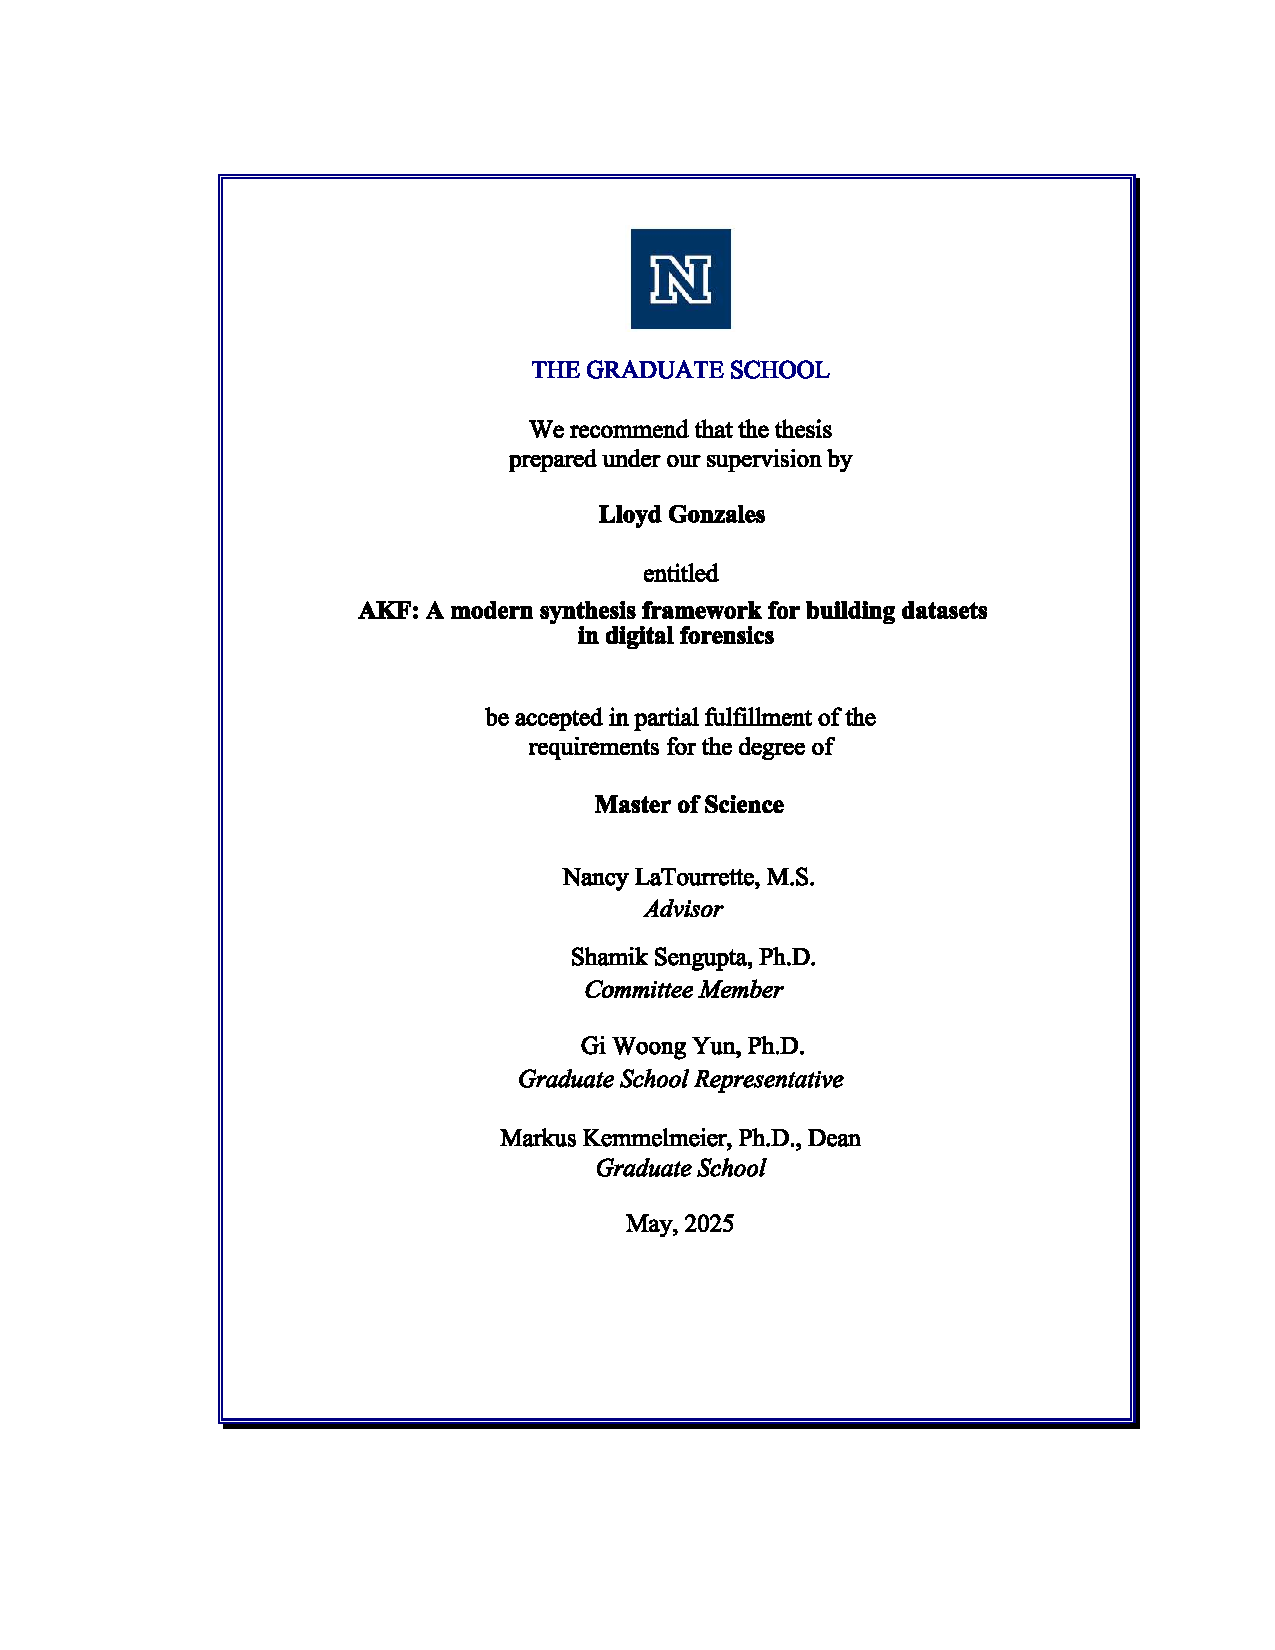
\includepdf[scale=1,pages=1, offset=0 0]{ms-committee-final}

% == Set page numbering style ============================================
\pagenumbering{roman}
\setcounter{page}{0}

% == Abstract ===========================================================
\newpage
\onehalfspace

\begin{abstract}

\thispagestyle{fancyplain}
\doublespacing
As our world becomes increasingly dependent on technology, the
advancement of digital forensics has become a key focus in the fight
against cybercrime. The forensic community depends on the availability
of disk images, network captures, and other forensic artifacts for
education, tool validation, and research. However, real-world datasets
often contain sensitive information that may be difficult to remove,
making them challenging to distribute publicly. As a result, researchers
and educators can encounter gaps in available datasets, typically leading to
the manual development of new datasets. While viable, this approach is
time-consuming and rarely produces datasets that accurately reflect
real-world scenarios suitable for comprehensive training and education.
In turn, there is ongoing research into forensic synthesizers, which
automate the process of creating unique, synthetic datasets
that can be publicly distributed without legal and other logistical
concerns.

This thesis introduces the \emph{\emph{automated kinetic framework}}, or
AKF, a modular synthesizer for creating and interacting with virtualized
environments to simulate human activity. AKF significantly improves upon
the designs and implementations of prior synthesizers while largely
maintaining feature parity and usability. Additionally, AKF leverages
the CASE standard to provide human- and machine-readable reporting,
exposing low-level dataset features in a searchable format. Finally, this thesis
describes options for leveraging generative AI to develop high-level
scenarios as well as individual artifacts. These contributions are
intended to improve the speed at which synthetic datasets can be created
and ensure the long-term usefulness of AKF-generated datasets and the
framework as a whole.
\end{abstract}

% == Set page number ====================================================
\setcounter{page}{2}
\doublespacing


% == Dedication ==========================================================

% \begin{center}

\section*{Dedication}

To those in the osu! tournament community, without whom I would have
never embarked on this journey;

To my numerous teachers and professors, especially Keith Lightfoot,
Rodney Rogers, Marc Miller, and Gabbi Bachand, whom I have limitless
appreciation and admiration for;

To those on the United States Cyber Team and the broader CTF
community for igniting my interest in digital forensics and supporting
me even when I flailed like a fish out of water;

And, of course, to my friends, family, and bed, who provided support and motivation.

% \end{center}

% == Acknowledgments ====================================================
\newpage

\section*{Acknowledgments}

I want to express my immense gratitude to Nancy LaTourrette for her
support, guidance, and mentorship throughout the development of this
thesis. This thesis would be nowhere without her ideas and experience,
and I am truly grateful and honored to have been able to work with her
throughout this thesis.

I would also like to thank Bill Doherty for reviewing a prior paper
from which some of this thesis's content is derived, as well as Bank Sombatsiri
for proofreading and providing feedback on this thesis.

I acknowledge the use of Grammarly and ChatGPT in making grammar and clarity
improvements during proofreading.


% == Table of contents ===================================================
\newpage
\renewcommand*\contentsname{Table of Contents}
\tableofcontents

\newpage
\listoftables

\newpage
\listoffigures

\newpage
\renewcommand{\lstlistlistingname}{List of Code Listings}
\lstlistoflistings

% == Set new page number style ===========================================
\newpage
\pagenumbering{arabic}
\setcounter{page}{1}
\linespread{2}

{{thesis_sub_here}}

%glossary & acronym lists
% \printglossary[type=\acronymtype]
% \printglossary

% \nocite{*}
\singlespacing
\printbibliography[heading=bibintoc, title={Bibliography}]
% \bibliography{thesis_bib}

\doublespacing
\appendix

\appendix

{{thesis_appendix_here}}

\end{document}